\documentclass[12pt,twoside]{article}
\usepackage{amsmath, amssymb}
\usepackage{amsmath}
\usepackage[active]{srcltx}
\usepackage{amssymb}
\usepackage{amscd}
\usepackage{makeidx}
\usepackage{amsthm}
\usepackage{algpseudocode}
\usepackage{algorithm}
\usepackage{natbib}
\usepackage{graphicx}
\usepackage{multirow}
\renewcommand{\baselinestretch}{1}
\setcounter{page}{1}
\setlength{\textheight}{21.6cm}
\setlength{\textwidth}{14cm}
\setlength{\oddsidemargin}{1cm}
\setlength{\evensidemargin}{1cm}
\pagestyle{myheadings}
\thispagestyle{empty}
\markboth{\small{Josu\'e David Hern\'andez Ram\'irez}}{\small{.}}
\date{}
\begin{document}
\centerline{\bf Introducción a las redes neuronales artificiales, Sem: 2021-1, 3CV3, Tarea 1, 30/09/2020}
\centerline{}
\centerline{}
\begin{center}
\Large{\textsc{Tarea 1: Ejercicios TLU's}}
\end{center}
\centerline{}
\centerline{\bf {Josu\'e David Hern\'andez Ram\'irez.}}
\centerline{}
\centerline{Escuela Superior de C\'omputo}
\centerline{Instituto Polit\'ecnico Nacional, M\'exico}
\centerline{$jhernandezr1605@alumno.ipn.mx$}
\newtheorem{Theorem}{\quad Theorem}[section]
\newtheorem{Definition}[Theorem]{\quad Definition}
\newtheorem{Corollary}[Theorem]{\quad Corollary}
\newtheorem{Lemma}[Theorem]{\quad Lemma}
\newtheorem{Example}[Theorem]{\quad Example}
\bigskip
% \textbf{Resumen:} Redactar de manera breve y concisa de que trata el trabajo presentado. Un
% s\'olo p\'arrafo.
% {\bf Palabras Clave:} Colocar de 3 a 5 palabras clave.
\section{Primer ejercicio}


    En este ejercicio usando el método manual, la solución que encontre fue
haciendo tanteo, me dí cuenta que el peso 2 que corresponde al eje de las
"X" tenía que estar lo mas cercano al punto (3,2), ya que en los casos
que estuve trabajando, entre mas alto su valor y menor valor del eje de las "Y"
los puntos a evaluar, ninguno se calsificaba entre una clase u otra. La fórmula
usada es:

$$x_{2} = - \frac{w_{1}}{w_{2}}x_{1} + \frac{\theta}{w_{2}}$$

    \begin{figure}[h!]
        \centering
        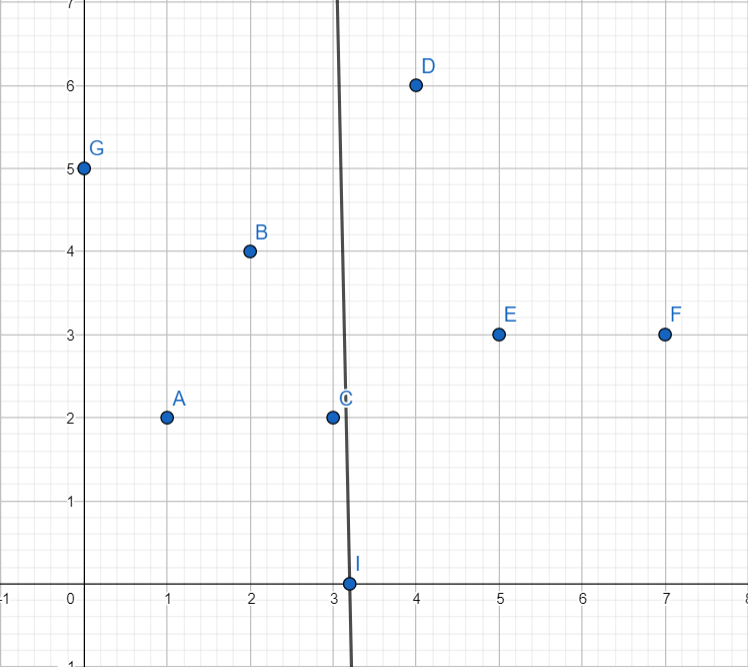
\includegraphics[scale=0.25]{./img/ejercicio1}
        \caption{Ejercicio 1}
        \label{fig:ejer1}
    \end{figure}

Como resultado obtuve la siguiente configuración de valores:
    \begin{enumerate}
        \item \textbf{$w_{1}$}= -100
        \item \textbf{$w_{2}$}= 3.2 
        \item \textbf{$\theta$}= 320 
    \end{enumerate}

    Asumiendo que el resultado sea $\geq 0$ pertenece a la clase 1 y
siendo $< 0$ era la clase 2, logrando hacer las calisificaciones y por ende, 
resolver el primer ejercicio.

\section{Segundo ejercicio}

    En este ejercicio, si pedí ayuda a compañeros, puesto que se me 
complicaba hacerlo por mi cuenta. Haciendo lluvia de ideas, llegamos
a la conclusión de usar la ecuación de la recta, que al aprecer es otro
modo mas efectivo para resolver el primer ejercicio.\\

Para lograr sacar el ejercicio, nos basamos en la TLU del XOR, así que, primero 
sacamos las pendientes de cada recta y asi obtuvimos sus pesos y el bias, teniendo
como resultado lo siguiente:\\

$$x_{2} = - \frac{w_{1}}{w_{2}}x_{1} + \frac{\theta}{w_{2}}$$\\

    \begin{figure}[h!]
        \centering
        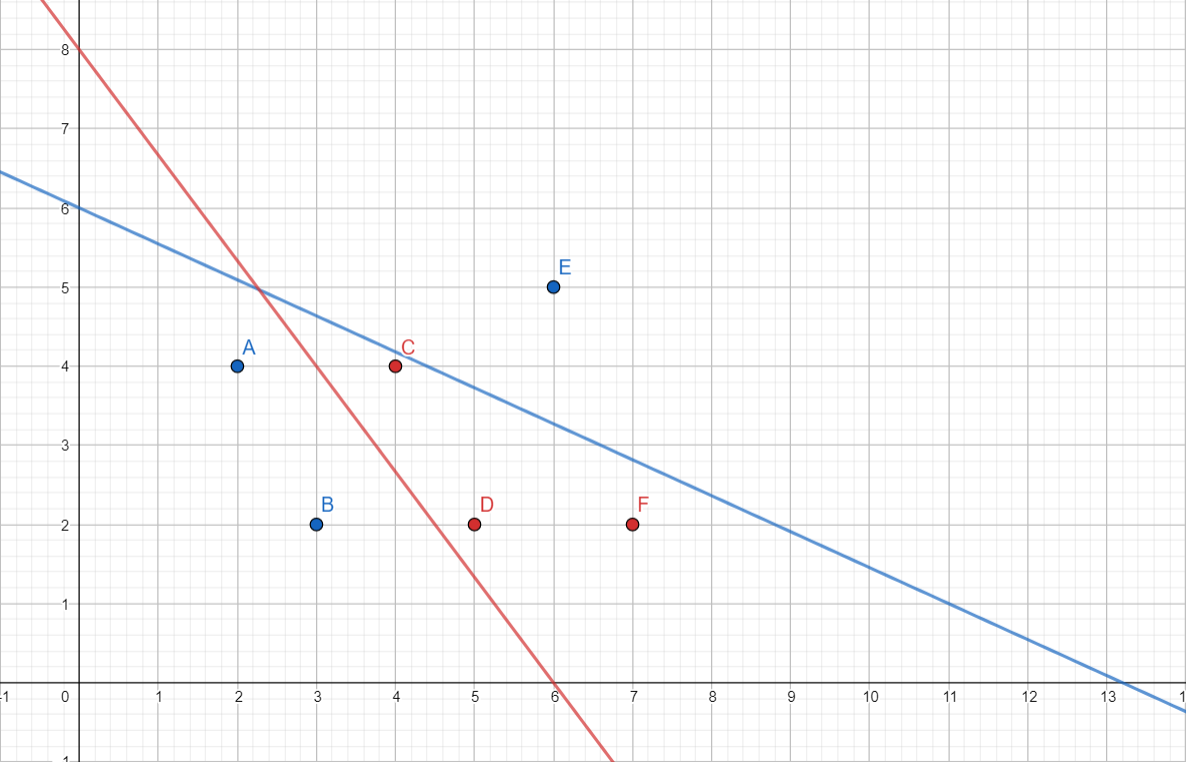
\includegraphics[scale=0.3]{./img/ejercicio2}
        \caption{Ejercicio 1}
        \label{fig:ejer2}
    \end{figure}

Para la recta uno, de color azul según la Figura \ref{fig:ejer2}:
\begin{enumerate}
    \item \textbf{$w_{1}$}= 5
    \item \textbf{$w_{2}$}= 11 
    \item \textbf{$\theta$}= -66 
\end{enumerate}

Para la recta dos, de color rojo según la Figura \ref{fig:ejer2}:

\begin{enumerate}
    \item \textbf{$w_{1}$}= 8
    \item \textbf{$w_{2}$}= 6 
    \item \textbf{$\theta$}= -48 
\end{enumerate}


Con base a los analisis que hicimos, nos dimos cuenta que la clase azul
cumple ciertas condiciones como lo son: que dos de ellas siempre van a 
estar abajo de la recta y una va a estar arriba de las dos rectas. Por otro
lado, la clase roja va a estar sobre una recta, en este caso, la recta roja 
y siempre va a estar por debajo de la línea azul, lo que nos reafirma que
podemos usar la configuración de la TLU para el XOR.\\

Por lo tanto, solo restaba calcular los pesos y el bias necesario para 
poder concluir la clasificación, teniendo como resultado la siguiente condición y
valores:

\begin{equation}
    f(a) = \left\{ \begin{array}{lcc}
        1 &   si  & a \geq 0 \\
        \\0 &  si & a < 0 \\
        \end{array}
    \right.
\end{equation}

\begin{enumerate}
    \item \textbf{$w_{1}$}= -1
    \item \textbf{$w_{2}$}= 1
    \item \textbf{$\theta$}= -1 
\end{enumerate}

\newpage
Teniendo la siguiente tabla:

\begin{table}[htbp]
    \centering
    \resizebox{10cm}{!}{
        \begin{tabular}{|r|r|r|r|r|r|r|r|}
            \hline
            \multicolumn{1}{|c|}{$x_{1}$} & \multicolumn{1}{c|}{$x_{2}$} & \multicolumn{1}{c|}{$r_{1}$} & \multicolumn{1}{c|}{$r_{2}$} & \multicolumn{1}{c|}{$S_{1}$} & \multicolumn{1}{c|}{$S_{2}$} & \multicolumn{1}{c|}{$r_{3}$} & \multicolumn{1}{c|}{$S_{3}$} \\ \hline
            2 & 4 & -12 & -8 & 0 & 0 & -1 & 0 \\ \hline
            6 & 5 & 19 & 30 & 1 & 1 & -1 & 0 \\ \hline
            3 & 2 & -18 & -12 & 0 & 0 & -1 & 0 \\ \hline
            4 & 4 & -2 & 8 & 0 & 1 & 0 & 1 \\ \hline
            5 & 2 & -19 & 4 & 0 & 1 & 0 & 1 \\ \hline
            7 & 2 & -9 & 20 & 0 & 1 & 0 & 1 \\ \hline
        \end{tabular}
    }
    \caption{Resultados del ejercicio 2.}
    \label{tabla:resultadosejercicio2}
\end{table}
Como se puede apreciar en la tabla \ref{tabla:resultadosejercicio2}
la arquitectura de una TLU para la compuerta lógica XOR fue bastante útil
en este ejercicio.\\

Tomando la experiencia del primer ejercicio, se usaron los pesos encotnrados
en cada recta para después, mediante el tanteo conseguir los pesos y el bias
para obtener los resultados deseados.

\section{Conclusiones}
Tomando en cuenta los resultados satisfactorios, es interesante ver como 
se aplican conocimientos básicos de geometría analítica se puede obtener
resultados interesantes.\\
Ayuda bastante aplicar los conceptos vistos en clase, para poder
comprender lo que se nos ha enseñado y visualizar como conceptos tan
básicos aplicados a una perspectiva diferente se puede llegar a interesantes
conclusiones.
\end{document}

